\section{Auswertung}
\label{sec:Auswertung}
 \subsection{Kennlinienschar einer Hochvakuumdiode}
 Es wurde von $I_{1}=1.9$ A bis $I_{5}=2.3$ A in $\Delta I=0.1$ A Schritten gemessen. Die Kennlinien sind in \autoref{b1} aufgetragen.
 \begin{figure}[H]
 \centering
 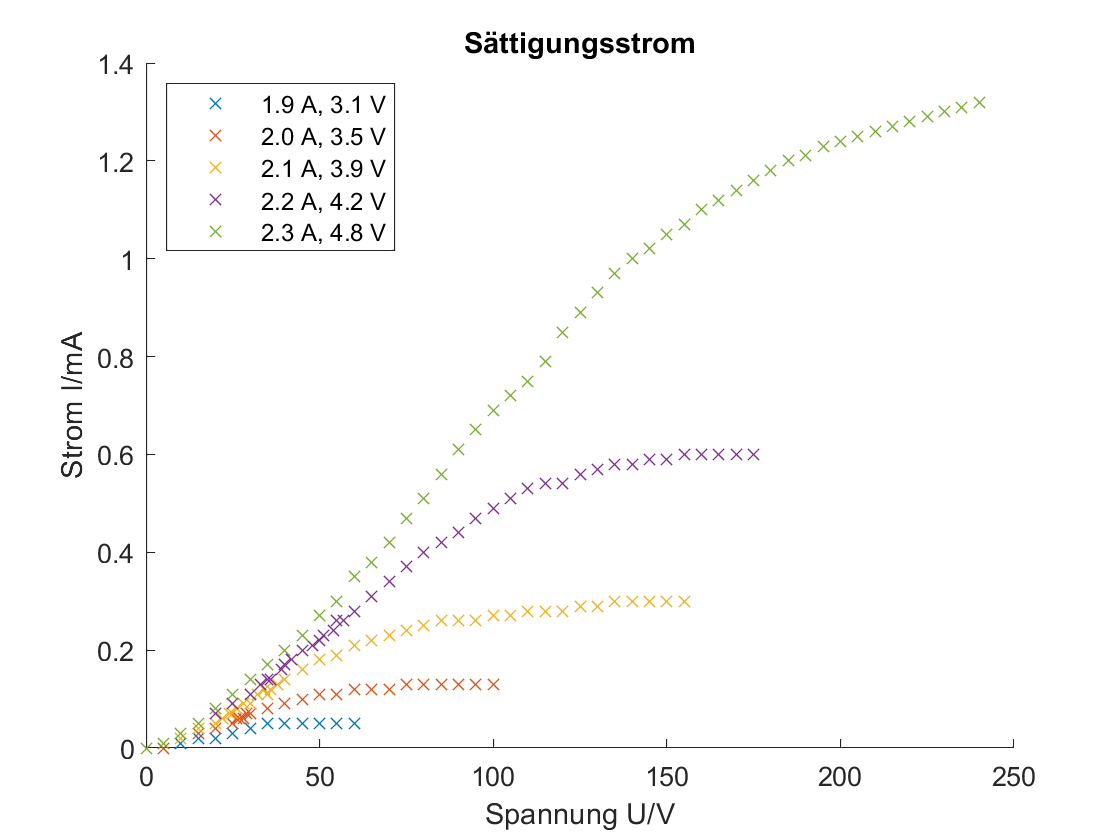
\includegraphics[width=8cm]{s.png}
 \caption{Sättigungsstrom I gegen Saugspannung bei voreingestellem Heizstrom.}
 \label{b1}
 \end{figure}
 Aus \autoref{b1} lassen sich die Sättigungsstörme aus \autoref{t1} ablesen. 
 \begin{table}[H]
  \centering
  \caption{Sättigungsströme $I_{s}$ zu den Heizspannungen $I_{i}$}
  \begin{tabular}{l|l}
  $I_{i}/A$& $I_{s}$/mA\\\hline
  $1.9$ & 0.05\\
  $2.0$ & 0.13\\
  $2.1$ & 0.30\\
  $2.2$ & 0.60\\
  $2.3$ & -\\\hline
  \end{tabular}
  \label{t1}
 \end{table}

 \subsection{Gültigkeitsbereich des Langmuir-Schottkyschen Raumladungsgesetzes}
 Da nur bis zu einem Heizstrom von $I=2.3$ A gemessen wurde, wird auch nur für diesen Strom der Gültigkeitsbereich ermittelt. Dazu wird der Strom gegen die Spannung auf
 \begin{equation*}
   I=a\cdot V^{b}
 \end{equation*}
 gefittet. Mit MATLAB ergeben sich die Werte
 \begin{align*}
   a&=(0.001526 \pm 0.000228)\ \frac{\textrm{W}}{\textrm{V}^2 \cdot\textrm{m}^2}\ \textrm{und}\\
   b&=(1.325 \pm 0.033)
 \end{align*}
 für die Parameter, wenn $U=110$ V als obere Grenze gewählt wird. Alle Spannungen unter $U=110$ V ergeben keine signifikante Änderung für $b$.
 
 \subsection{Anlaufstromgebiet der Kathode}
 \label{sec:t1}
 Bei dem Anlaufstrom ist zu beachten, dass das Nanoampermeter einen Innenwiderstand von $R=1\ \textrm{M}\Omega$ besitzt, sodass die Spannung von $U$ auf
 \begin{equation*}
   U_{A}=U+R\cdot I
 \end{equation*}
 korrigiert werden muss. Dadurch ergeben sich die korrigierten Spannungen $U_{A}$ aus \autoref{t3}.
 \begin{table}[H]
 \centering
 \caption{Ausgangsspannungen und -ströme und die korrigierte Spannung}
 \begin{tabular}{l|l|l|l|l|l}
 U/V & I/nA & $U_{A}$/V & U/V & I/nA & $U_{A}$/V\\\hline
 0.05 & 700 & 0.75 & 0.55 & 75 & 0.625\\
 0.10 & 500 & 0.60 & 0.60 & 60 & 0.66\\
 0.15 & 400 & 0.55 & 0.65 & 49 & 0.699\\
 0.20 & 250 & 0.45 & 0.70 & 38 & 0.738\\
 0.25 & 310 & 0.56 & 0.75 & 31 & 0.781\\
 0.30 & 240 & 0.54 & 0.80 & 26 & 0.826\\
 0.35 & 180 & 0.53 & 0.85 & 21 & 0.871\\
 0.40 & 140 & 0.49 & 0.90 & 17 & 0.917\\
 0.45 & 100 & 0.55 & 0.95 & 14 & 0.964\\
 0.50 & 75 & 0.575 & - & - & -\\\hline
 \end{tabular}
 \label{t3}
 \end{table}
 Dann lässt sich aus \eqref{eq:richardson} die Formel 
 \begin{equation*}
   \textrm{ln}(I)=a\cdot U+b
 \end{equation*}
 für den Fit bestimmen, der im Graph aus \autoref{fit2} abgebildet wurde. Mit MATLAB ergeben sich für die Parameter
 \begin{align*}
   a&=-\frac{e}{k_{B}\cdot T}=(-5.9 \pm 2.73)\ \frac{1}{\textrm{V}}\ \textrm{und}\\
   b&=(8.447 \pm 1.865)\ \textrm{A},
 \end{align*}
 für den Fit.
 \begin{figure}[H]
 \centering
 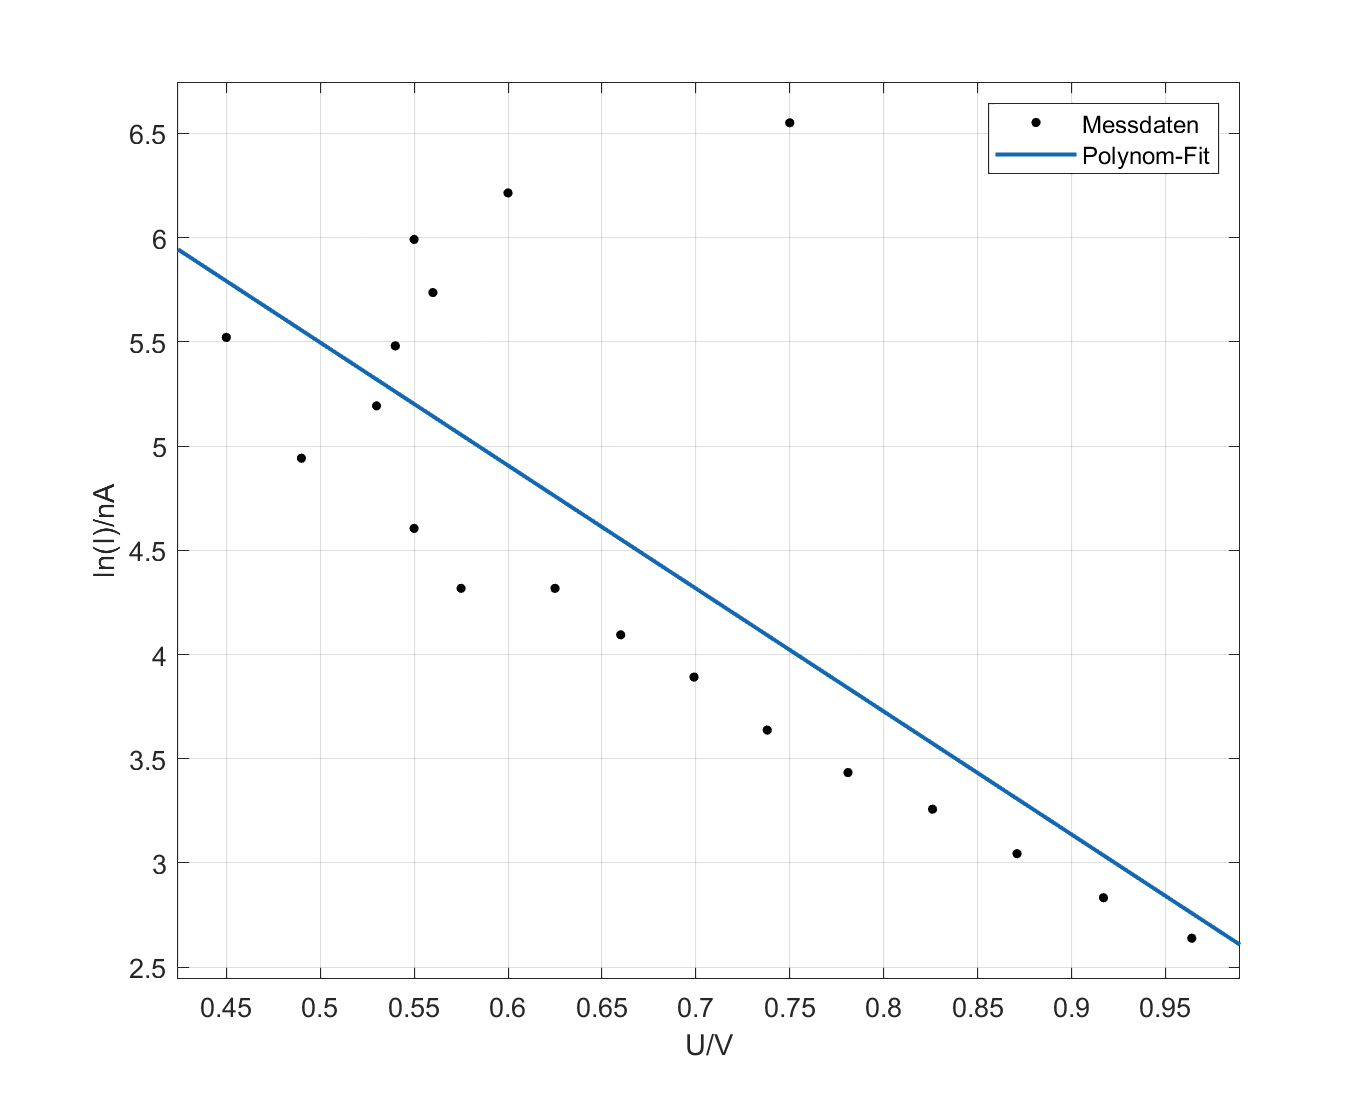
\includegraphics[width=8cm]{linfit.png}
 \caption{Fit für den logarithmierten Strom}
 \label{fit2}
 \end{figure}
 Durch Umstellen ergibt sich die Kathodentemperatur 
 \begin{equation*}
   T=-\frac{e}{k_{B}\cdot a}=1967.58\ \textrm{K}
 \end{equation*}
 für den Anlaufstrom. 

 \subsection{Kathodentemperatur T und Austrittsarbeit für Wolfram}
 \label{sec:T2}
 Die Kathodentemperatur $T$ kann aus der Leistungsbilanz des Heizstromfadens ermittelt werden. Aus dem Energiesatz 
 \begin{equation*}
   P_{Zu}=P_{Str}+P_{WL}
 \end{equation*}
 mit der zugeführten Leistung $P_{Zu}=U_{H}\cdot I_{H}$, der Strahlungsleistung $P_{Str}=f\eta\sigma T^4$ und der Wärmeleitung $P_{WL}=1$ W, dem Emissionsgrad $\eta=0.28$ der Oberfläche, der Strahlungskonstante $\sigma=5.7\cdot 10^{-12} \frac{\textrm{W}}{\textrm{cm}^2\textrm{K}^4}$ und der emittierenden Kathodenoberfläche $f=0.35 \textrm{cm}^2$  kann die Temperatur
 \begin{equation*}
   T=\left(\frac{I_{H}\cdot U_{H}-P_{WL}}{f\eta\sigma}\right)^{\frac{1}{4}}
 \end{equation*}
 ermittelt werden. Durch Einsetzen der Heizströme und -Spannungen ergeben sich die Temperaturen in \autoref{t2}.
 \begin{table}[H]
 \centering
 \caption{Temperaturen zu den Heizströmen und -spannungen.}
 \begin{tabular}{l|l|l}
 $U_{H}/V$ & $I_{H}$/A & T/K\\ \hline
 3.1 & 1.9 & 1720.09\\
 3.5 & 2.0 & 1810.35\\
 3.9 & 2.1 & 1894.12\\
 4.2 & 2.2 & 1959.78\\
 4.8 & 2.3 & 2059.01
 \end{tabular}
 \label{t2}
 \end{table}
 Wird jetzt die Richardson-Gleichung nach $e\phi$ umgestellt, ergibt sich 
 \begin{equation*}
 e\phi=-k_{B}T\textrm{ln}(\frac{I_{s}h^3}{4\pi f em_{e}k_{B}^2T^2})
 \end{equation*}
 die Austrittsarbeit, mit $f=35\ \textrm{mm}^2$. Für die vier ermittelten Sättigungsströme und Temperaturen wurden die Austrittsarbeiten 
 \begin{align*}
   e\phi_{1}&=3.548\ \textrm{eV},\\
   e\phi_{2}&=3.601\ \textrm{eV},\\
   e\phi_{3}&=3.646\ \textrm{eV}\ \textrm{und}\\
   e\phi_{4}&=3.667\ \textrm{eV}\\
 \end{align*}
 berechnet. Im Mittel ergibt sich 
 \begin{equation*}
   \bar{e\phi}=(3.616 \pm 0.026)\ \textrm{eV}
 \end{equation*}
für die Austrittsarbeit.

